\documentclass[11pt]{amsart}
\usepackage[utf8]{inputenc}
\usepackage[T1]{fontenc}
\usepackage{lmodern}
\usepackage{amssymb,amsmath,amsthm}
\usepackage[margin=1.1in]{geometry}
\usepackage{booktabs,array,enumitem}
\usepackage[dvipsnames]{xcolor}
\usepackage{tikz}
\usetikzlibrary{positioning,arrows.meta}
\usepackage[colorlinks=true,linkcolor=blue!50!black,citecolor=green!40!black,urlcolor=blue!50!black]{hyperref}

\newcommand{\Q}{\mathbb{Q}}
\newcommand{\cO}{\mathcal{O}}
\newcommand{\St}{\mathrm{St}}
\newcommand{\stat}[1]{\textsc{[#1]}}
\newcommand{\Vol}{\mathrm{Vol}}

\title[Research summary]{Beyond square-free conductor in the supersingular $p=5$ converse theorem: question, research path, results and prospects\\[4pt]\normalfont\small A research summary}
\date{November 2026 (draft). Technical details: companion note \emph{``What is new''} (NEW\_RESULTS\_EN.pdf).}

\raggedbottom
\begin{document}
\begin{abstract}
This summary explains, for a specialist reader, the question we studied, why it matters, the path we followed (including dead ends), what we obtained, and what could follow. Each statement carries one of the following labels:
\begin{itemize}
\item \stat{proved}: complete argument given;
\item \stat{confirmed}: confirmed by the author of the work concerned;
\item \stat{deduction}: complete outline, awaiting expert check;
\item \stat{open}.
\end{itemize}
The work was carried out by an amateur with extensive assistance from an AI system (Claude). Every cited statement was checked against the source.
\end{abstract}
\maketitle

\section{The question}
Bhargava, Skinner and Zhang proved that at least $66.48\%$ of elliptic curves over $\Q$, ordered by height, satisfy the Birch--Swinnerton-Dyer rank conjecture [BSZ]. Later $p$-converse theorems [BSTW], [Cas] raise this to about $67\%$. The method combines the average size $6$ of $5$-Selmer groups in large families with \emph{$p$-converse theorems}: Selmer rank $r\le1$ implies analytic rank $r$.

[BSZ, \S4] already observe that if their Theorem~9 could be extended to curves with \emph{supersingular} reduction at $p$ ([BSZ, Remark~10]), the bound would rise to $79.7\%$. [BSTW, Thm.~1.6, 12.3] supply this extension for $p=5$, but only when the conductor $N$ is \emph{square-free}. Most curves of the supersingular family $\{5\mid A,\ 5\nmid B\}$ have additive reduction at $2$ or $3$ (in the [BSZ] normalization, about $92\%$ are supercuspidal at $2$), so the square-free hypothesis loses almost all of the expected gain.

\medskip\noindent\textbf{Question.} \emph{Can the square-free hypothesis be removed from the supersingular $p=5$ converse theorems, at least at the primes $2$ and $3$? If so, how far does the bound rise?}

The authors themselves describe the hypothesis as removable: ``The hypothesis that $N$ be squarefree is carried over from [CLW22], and it should be removable with some more work'' [CLW26, \S1.5(3)].

\section{Where the obstruction lies}
\begin{center}
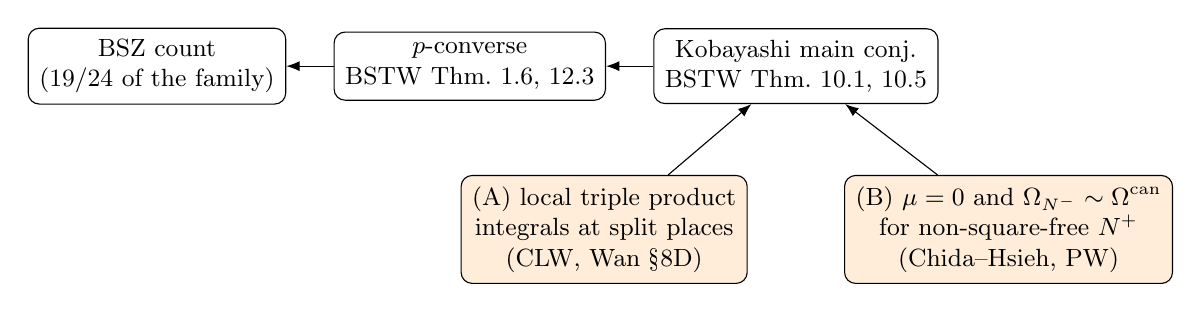
\begin{tikzpicture}[node distance=7mm and 6mm, every node/.style={draw, rounded corners, align=center, font=\small, inner sep=4pt}]
\node (bsz) {BSZ count\\ ($19/24$ of the family)};
\node (conv) [right=of bsz] {$p$-converse\\ BSTW Thm.~1.6, 12.3};
\node (k) [right=of conv] {Kobayashi main conj.\\ BSTW Thm.~10.1, 10.5};
\node (A) [below left=9mm and -12mm of k, fill=orange!15] {(A) local triple product\\ integrals at split places\\ (CLW, Wan \S8D)};
\node (B) [below right=9mm and -12mm of k, fill=orange!15] {(B) $\mu=0$ and $\Omega_{N^-}\sim\Omega^{\mathrm{can}}$\\ for non-square-free $N^+$\\ (Chida--Hsieh, PW)};
\draw[-{Latex}] (conv) -- (bsz);
\draw[-{Latex}] (k) -- (conv);
\draw[-{Latex}] (A) -- (k);
\draw[-{Latex}] (B) -- (k);
\end{tikzpicture}
\end{center}
Reading the whole chain shows that ``$N$ square-free'' is used in exactly two places (established by reading the sources):
\begin{enumerate}[label=(\Alph*)]
\item \emph{Local triple product integrals}: ``The square-free-ness was assumed in loc.\ cit.\ for explicit calculation of local triple product periods'' [BSTW, fn.~20].
\item \emph{The $\mu$-invariant and the comparison of periods} in [BSTW, Thm.~10.5], which rely on [PW] (square-free level).
\end{enumerate}

\section{Research path}
\begin{enumerate}[label=\arabic*.]
\item \textbf{(A), first attempt.} We computed the local integral for supercuspidal $\pi_v$ with the local data of [CLW, \S5.6]. We found an obstruction (route 1). We then found that Fouquet--Wan [FW, Prop.~7.27, Cor.~7.28] treat exactly this case with a different choice of data: the newvector, and characters with $\chi_{h,i}\chi_{\theta,i}$ unramified. We re-proved their computation for all $\ell$, including $\ell=2$.
\item \textbf{A consistency check that failed.} To understand why the data of [CLW] differ from those of [FW], we tested [Wan, Lemmas 8.13--8.17] numerically. Lemma~8.13 checked out. The support statement of Lemma~8.14 did not.
\item \textbf{Understanding the failure.} A representation-theoretic criterion (Casselman's newform theory) shows that, with the vectors of Lemma~8.17, the local integral vanishes identically. We then established, from the Schwartz functions in [CLW, \S7.7], that the vectors of $\theta$ and $h$ have the same orientation, as Wan's Remark~8.19 states. We checked that the published version of [CLW] is unchanged on all these points.
\item \textbf{A repair.} Replacing the newvector by the vector with Kirillov function $A^{-1}1_{\cO^\times}$, and matching the type of the auxiliary data, gives a non-zero constant for \emph{every} generic $\pi_v$. The proof uses only the support of this vector in the Kirillov model.
\item \textbf{(B).} We transcribed [CH, \S5--6] for arbitrary $N^+$, with the crystalline condition of [Tay06, \S2] in place of the ordinary one, as already suggested in [KO, Rem.~6.6]. This uncovered a minimality issue at $2$ and $3$ that the square-free case never meets.
\item \textbf{Adversarial review.} We ran two rounds of hostile self-review: $26$ objections, then $10$ more. We checked every reference against the source, and verified on the web that nothing has superseded the work.
\item \textbf{Contact with the author.} X.~Wan confirmed the supercuspidal case (below).
\end{enumerate}

\section{Results}
\begin{center}\small
\begin{tabular}{p{7.4cm}p{2.3cm}p{4.2cm}}
\toprule
Result & Status & Comment\\ \midrule
R1. The support statement of [Wan, Lemma~8.14] (ANT 2020) is false for every $s>t$: $\Phi(n(\varpi^{s-t-1}))=-\Phi(1)/(q-1)\neq0$. & \stat{proved} & three-line proof; three independent numerical checks\\
R2. With the vectors of [Wan, Lemma~8.17], Ichino's local integral is $0$ (except $t_1=0$, $s=1$). & \stat{proved} & short proof via [Cas73, Thm.~1]; independent of R1\\
R3. With the local data (4) of [CLW] (published version, p.~39, 78), the local integral vanishes at split places where $\pi_v$ is ramified, already for square-free $N$. & \stat{deduction} & rests on the identification of the local vectors stated in [Wan, Rem.~8.19]\\
R4. Supercuspidal split places: the choice of [FW, Prop.~7.27] works. & \stat{confirmed} & X.~Wan, private communication (citation subject to his permission)\\
R5. For every generic $\pi_v$, the vector $\phi_A$ with matching data gives $I_v=\Vol(K_{t_1})\neq0$, independent of the family. & \stat{proved} modulo [Wan, Lemma~8.13] & numerical checks at $\ell=2,3$\\
R6. (B) for arbitrary $N^+$ at minimal level, crystalline version of [CH, Prop.~6.8]. & \stat{deduction} & steps traced in [Tay06, \S2]\\
R7. Non-minimal configurations (E1)--(E3) at $2,3$ are genuine (standard definition [KO, Def.~3.5]). & \stat{proved} & excluded from the count\\
R8. The twist $g_K$ at primes dividing $D_K$ (rank $1$) is left open in [BSTW] as well. & \stat{open} & inherited point\\ \bottomrule
\end{tabular}
\end{center}

\section{What this could give}
\begin{center}\small
\begin{tabular}{p{8.3cm}l}
\toprule
Scenario & proportion\\ \midrule
Current (BSZ + BSTW + Castella) & $67.02\%$\\
(A) all types via R4/R5, (B) via R6, excluding (E1)--(E3); conditional on R8 and on expert validation & $\mathbf{78.61\%}$\\
Same, with (E1)--(E3) recovered (via [Dia97b] and twisting) & $79.03\%$\\
Also using $p=3$ (suggested in [BSZ, \S4]) & $>80\%$ (not computed)\\ \bottomrule
\end{tabular}
\end{center}
\noindent There are also two by-products, independent of the bound:
\begin{itemize}
\item R1--R3 bear on a published local computation used by [CLW], and through it by [BSTW] and [CLW26].
\item R5 gives a uniform replacement of that computation.
\end{itemize}

\section{What we would like to know}
\begin{enumerate}
\item Are R2 and R3 correct, i.e.\ are the vectors of Lemma~8.17 those used at split places, and does R5 restore the argument for principal series and Steinberg places?
\item Is condition (4) of [CLW] at the auxiliary prime $\ell$ compatible with the twist by $\nu$?
\item In (B), is [CH, Lemma~6.5] correct in the configurations (E2) and (E3)? How should the twist $g_K$ at $\ell\mid D_K$ be handled (R8)?
\end{enumerate}
All of this is independent of any Riemann hypothesis: the arguments are local and $p$-adic.

\begin{thebibliography}{BSTW}\small
\bibitem[BSZ]{BSZ} M.~Bhargava, C.~Skinner, W.~Zhang, \emph{A majority of elliptic curves over $\Q$ satisfy the BSD conjecture}, arXiv:1407.1826.
\bibitem[BSTW]{BSTW} A.~Burungale, C.~Skinner, Y.~Tian, X.~Wan, \emph{Zeta elements for elliptic curves and applications}, arXiv:2409.01350.
\bibitem[Cas]{Cas} F.~Castella, \emph{Exceptional zeros for Heegner points and $p$-converse to the theorem of Gross--Zagier and Kolyvagin}, arXiv:2409.01360.
\bibitem[Cas73]{Cas73} W.~Casselman, \emph{On some results of Atkin and Lehner}, Math.\ Ann.\ 201 (1973).
\bibitem[CH]{CH} M.~Chida, M.-L.~Hsieh, \emph{Special values of anticyclotomic $L$-functions for modular forms}, J.\ reine angew.\ Math.\ 741 (2018).
\bibitem[CLW]{CLW} F.~Castella, Z.~Liu, X.~Wan, \emph{Iwasawa--Greenberg main conjecture for nonordinary modular forms and Eisenstein congruences on $GU(3,1)$}, Forum Math.\ Sigma 10 (2022), e110.
\bibitem[CLW26]{CLW26} F.~Castella, Z.~Liu, X.~Wan, \emph{Kato's main conjecture for nonordinary modular forms}, arXiv:2608.29470.
\bibitem[Dia97b]{Dia97b} F.~Diamond, \emph{The Taylor--Wiles construction and multiplicity one}, Invent.\ Math.\ 128 (1997).
\bibitem[FW]{FW} O.~Fouquet, X.~Wan, \emph{The Iwasawa main conjecture for universal families of modular motives}, arXiv:2107.13726.
\bibitem[KO]{KO} C.-H.~Kim, K.~Ota, \emph{On the quantitative variation of congruence ideals and integral periods of modular forms}, arXiv:1905.02926.
\bibitem[PW]{PW} R.~Pollack, T.~Weston, \emph{On anticyclotomic $\mu$-invariants of modular forms}, Compos.\ Math.\ 147 (2011).
\bibitem[Tay06]{Tay06} R.~Taylor, \emph{On the meromorphic continuation of degree two $L$-functions}, Doc.\ Math.\ (2006).
\bibitem[Wan]{Wan} X.~Wan, \emph{Iwasawa main conjecture for Rankin--Selberg $p$-adic $L$-functions}, Algebra Number Theory 14 (2020), 383--483.
\end{thebibliography}
\end{document}
